<<<<<<< 748b67fd60b26d45750e10209255345ebe612814

\section{Zielsetzung}
In diesem Versuch soll der Wärmetransport zwischen zwei Wärmeresevoiren untersucht werden.
Normalerweise wird in einem abgeschlossenen System die Wärmeenergie von dem wärmeren Resevoir zum
kälteren Reservoir transportiert. Im folgenden soll der Wärmefluss umgekehrt werden, also vom
kälteren Reservoir zum wärmeren. Dies ist nur möglich, wenn zusätzliche Energie
aufgewendet wird.

\section{Theorie}
\subsection{Die Wärmepumpe}
Bei einer Wärmepumpe wird ein reales Gas als Transportmedium verwendet. Dieses transportiert die
Wärme in Form von Phasenumwandlungsenergie, anders ausgedrückt: das Gas nimmt beim
Verdampfen Wärme auf und gibt diese beim Kondensieren wieder ab.
Daher sind Gase mit einer möglichst hohen Kondersationswärme gut geeignet.
\begin{figure}[H]
  \centering
  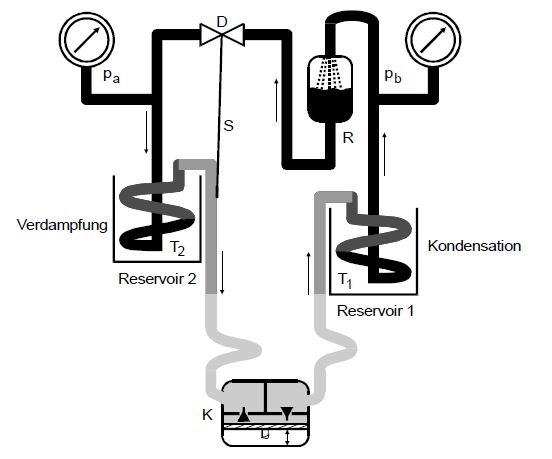
\includegraphics[height=8cm]{Pumpe.JPG}
  \caption{Aufbau einer Wämepumpe ($p_{b}>p_{a}$, $T_{1}>T_{2}$)}
  \cite{skript}.
  \label{fig:pumpe}
\end{figure}
Bei der Temperatur $T_{1}$ und dem Druck $p_{b}$ ist das Gas flüssig, nachdem es das Drosselventil D durchströmt
hat, verdampft das Gas im Reservoir 2 aufgrund des gernigen Drucks $p_{a}$. Dabei wird dem
Reservoir 2 die Verdampfungswärme $L$ pro Gramm Substanz entzogen, also gibt Reservoir 2 die Wärme ab und ist
damit das kältere Reservoir. Im Kompressor, der für eine Mediumskreislauf sorgt, wird das Gas nun
adiabatisch komprimiert, wobei es sich stark erwärmt und aufgrund des steigenden Drucks wieder verflüssigt.
Bei der Kondensation des Gases wird die Kondensationswärme L pro Gramm an das Reservoir 1 abgegeben, wodurch sich
dieses erwärmt.\\
Für den reibungsfreien Ablauf werden weitere Apparaturen benötigt, dazu zählt der Reiniger $R$, der
die übrigen Gasblasen aus dem verflüssigten Gas entfernt, sowie die Steuervorrichtung $S$.
Diese sorgt dafür, dass keine Flüssigkeitsreste des Gases in den Kompressor gelangen.
Außerdem muss die Durchlässigkeit des Drosselventils gesteuert werden, dies geschieht über
die Temperaturdifferen am Ein- und Ausgang der Reservoires 2.

\subsection{Kenngrößen der Wärmepumpe}
Bei einer realen Wärmepumpe sind folgende Kenngrößen von besonderem Interesse:
\begin{itemize}
  \item Güteziffer
  \item Massendurchsatz $\frac{dm}{dt}$ des Transportmediums
  \item Wirkungsgrad des Kompressors.
\end{itemize}

Aus dem zweiten Hauptsatz der Thermodynamik folgt unter der Annahme, dass sich die Temperaturen
$T_{1}$ und $T_{2}$ der Reservoire praktisch nicht ändern für den realen, irreversiblen Fall die Relation
\begin{equation}
  \frac{Q_{1}}{T_{1}}-\frac{Q_{2}}{T_{2}}>0.
  \label{eqn:QT}
\end{equation}
Wobei $Q_{1}$ die vom Transportmedium an das wärmere Reservoir abgegebene Wärmemenge bezeichnet und
$Q_{2}$ die vom kälteren Wärmereservoir aufgenommene Wärmemenge.

Eine wichtige Größe zur Beschreibung der Wärmepumpe ist die Güteziffer $\nu$, sie ist definiert
als das Vehältnis der transportieren Wärmemenge $Q_{1}$ zur geleisteten Arbeit $A$:
\begin{equation}
  \nu=\frac{Q_{1}}{A}.
  \label{eqn:güte}
\end{equation}
Mit dem ersten Hauptsatz der Thermodynamik lässt sich $Q_{1}$ als $Q_{1}=Q_{2}+A$ schreiben.\\
Unter der Verwendung von Gleichung \ref{eqn:QT} lässt sich die ideale Güteziffer als
\begin{equation}
  \nu_{id}=\frac{T_{1}}{T_{1}-T_{2}}
  \label{eqn:güte2}
\end{equation}
schreiben. Aus dieser Gleichung lässt sich folgender Zusammenhang folgern:
Je kleiner die Temperaturdifferenz zwischen den Reservoiren ist, desto weniger Arbeit muss
die Pumpe leisten.

Aus der Messreihe $T_{1}$ wird der Differenzenquotient $\Delta T_{1}/\Delta t$ bestimmt,
woraus zunächst eine Relation für $\frac{\Delta Q_{1}}{\Delta t}$ bestimmt wird.
\begin{equation}
  \frac{\Delta Q_{1}}{\Delta {t}}=(m_{1}c_{w}+m_{k}c_{k})\frac{\Delta T_{1}}{\Delta t}
\end{equation}
Hiebei bezeichnet $m_{1}c_{w}$ die Wärmekapazität des Wassers in Reservoir 1 und $m_{k}c_{k}$ die
Wärmekapazität der Kupferschlange, in der sich das Gas befindet und des Eimers, der das Wasserreservoir darstellt.\\
Mit der Größe $N$ als über das Zeitintervall $\Delta t$ gemittelte Leistungsaufnahme des Kompressors
kann folgende Formel für die Güteziffer bestimmt werden.
\begin{equation}
  \nu = \frac{\Delta Q_{1}}{\Delta t N}.
  \label{eqn:güte3}
\end{equation}

Aus der Messreihe $T_{2}$ wird ebenfalls der Differenzenquotient $\Delta T_{2}/\Delta t$
bestimmt, um folgende Relation zu erhalten:
\begin{equation}
  \frac{\Delta Q_{2}}{\Delta {t}}=(m_{2}c_{w}+m_{k}c_{k})\frac{\Delta T_{2}}{\Delta t}.
\end{equation}
Hier beschreibt $\Delta Q_{2}/{\Delta t}$ die pro Zeiteinheit aus dem Wärmereservoir 2
entnommene Wärmemenge.
Da dem Reservoir die Wärmemenge durch Verdampfen entzogen wird, wird pro Zeit- und Masseneinheit
die Verdampfungswärme $L$ verbraucht. Damit folgt die Relation
\begin{equation}
  \frac{\Delta Q_{2}}{\Delta t}= L \frac{\Delta m}{\Delta t}.
  \label{eqn:masse}
\end{equation}
Wenn die Verdampfungswärem $L $ bekannt ist, kann so der Massendurchsatz $\frac{dm}{dt}$ des Transportmediums
bestimmt werden.

Um die mechanisch Kompressionsleistung $N_{mech}$ zu bestimmen, wird zunächst die
Arbeit $A_{m}$ des Kompressors definiert, die verrichtet wird, wenn ein Gasvolumen von $V_{a}$ zu $V_{b}$
komprimiert wird:
\begin{equation}
  A_{m}= -\int_{V_{a}}^{V_{b}} p dV.
\end{equation}
Für eine adiabatische Kompression gilt:
\begin{equation}
  p_{a}V_{a}^{(\kappa)}=p_{b}V_{b}^{(\kappa)}=pV^{(\kappa)},
\end{equation}
und mit der Definition $N_{mech}=\frac{dA_{m}}{dt}$ folgt für die mechanische Kompressionsleistung
\begin{equation}
  N_{mech}= \frac{1}{\kappa-1}\Biggl(p_{b}\sqrt[\kappa]{\frac{p_{a}}{p_{b}}}-p_{a}\Biggr)\frac{\Delta V_{a}}{\Delta }=\frac{1}{\kappa-1}\Biggl(p_{b}\sqrt[\kappa]{\frac{p_{a}}{p_{b}}}-p_{a}\Biggr)\frac{\Delta m}{\rho \Delta t}
 \label{eqn:Nmech}
\end{equation}
wobei $\rho$ die Dichte des Gases beschreibt und $\kappa$ die Molwärmen $C_{P}$ und $C_{V}.

\label{sec:Theorie}

%\cite{sample}
||||||| merged common ancestors

\section{Zielsetzung}
In diesem Versuch soll der Wärmetransport zwischen zwei Wärmeresevoiren untersucht werden.
Normalerweise wird in einem abgeschlossenen System die Wärmeenergie von dem wärmeren Resevoir zum
kälteren Reservoir transportiert. Im folgenden soll der Wärmefluss umgekehrt werden, also vom
kälteren Reservoir zum wärmeren. Dies ist nur möglich, wenn zusätzliche Energie
aufgewendet wird.

\section{Theorie}
\subsection{Die Wärmepumpe}
Bei einer Wärmepumpe wird ein reales Gas als Transpurtmedium verwendet. Dieses transportiert die
Wärme in Form von Phasenumwandlungsenergie, anders ausgedrückt: das Gas nimmt beim
Verdampfen Wärme auf und gibt diese beim Kondensieren wieder ab.
Daher sind Gase mit einer möglichst hohen Kondersationswärme gut geeignet.
\begin{figure}[H]
  \centering
  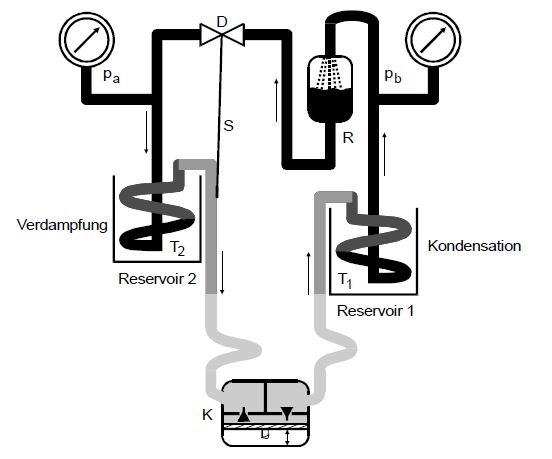
\includegraphics[height=8cm]{Pumpe.JPG}
  \caption{Aufbau einer Wämepumpe ($p_{b}>p_{a}$, $T_{1}>T_{2}$)}
  \cite{skript}.
  \label{fig:pumpe}
\end{figure}
Bei der Temperatur $T_{1}$ und dem Druck $p_{b}$ ist das Gas flüssig, nachdem es das Drosselventil D durchströmt
hat, verdampft das Gas im Reservoir 2 aufgrund des gernigen Drucks $p_{a}$. Dabei wird dem
Reservoir 2 die Verdampfungswärme $L$ pro Gramm Substanz entzogen, also gibt Reservoir 2 die Wärme ab und ist
damit das kältere Reservoir. Im Kompressor, der für eine Mediumskreislauf sorgt, wird das Gas nun
adiabatisch komprimiert, wobei es sich stark erwärmt und aufgrund des steigenden Drucks wieder verflüssigt.
Bei der Kondensation des Gases wird die Kondensationswärme L pro Gramm an das Reservoir 1 abgegeben, wodurch sich
dieses erwärmt.\\
Für den reibungsfreien Ablauf werden weitere Apparaturen benötigt, dazu zählt der Reiniger $R$, der
die übrigen Gasblasen aus dem verflüssigten Gas entfernt, sowie die Steuervorrichtung $S$.
Diese sorgt dafür, dass keine Flüssigkeitsreste des Gases in den Kompressor gelangen.
Außerdem muss die Durchlässigkeit des Drosselventils gesteuert werden, dies geschieht über
die Temperaturdifferen am Ein- und Ausgang der Reservoires 2.

\subsection{Kenngrößen der Wärmepumpe}
Bei einer realen Wärmepumpe sind folgende Kenngrößen von besonderem Interesse:
\begin{itemize}
  \item Güteziffer
  \item Massendurchstz $\frac{dm}{dt}$ des Transportmediums
  \item Wirkungsgrad des Kompressors.
\end{itemize}

Aus dem zweiten Hauptsatz der Thermodynamik folgt unter der Annahme, dass sich die Temperaturen
$T_{1}$ und $T_{2}$ der Reservoire praktisch nicht ändern für den realen, irreversiblen Fall die Relation
\begin{equation}
  \frac{Q_{1}}{T_{1}}-\frac{Q_{2}}{T_{2}}>0.
  \label{eqn:QT}
\end{equation}
Wobei $Q_{1}$ die vom Transportmedium an das wärmere Reservoir abgegebene Wärmemenge bezeichnet und
$Q_{2}$ die vom kälteren Wärmereservoir aufgenommene Wärmemenge.

Eine wichtige Größe zur Beschreibung der Wärmepumpe ist die Güteziffer $\nu$, sie ist definiert
als das Vehältnis der transportieren Wärmemenge $Q_{1}$ zur geleisteten Arbeit $A$:
\begin{equation}
  \nu=\frac{Q_{1}}{A}.
  \label{eqn:güte}
\end{equation}
Mit dem ersten Hauptsatz der Thermodynamik lässt sich $Q_{1}$ als $Q_{1}=Q_{2}+A$ schreiben.\\
Unter der Verwendung von Gleichung \ref{eqn:QT} lässt sich die ideale Güteziffer als
\begin{equation}
  \nu_{id}=\frac{T_{1}}{T_{1}-T_{2}}
  \label{eqn:güte2}
\end{equation}
schreiben. Aus dieser Gleichung lässt sich folgender Zusammenhang folgern:
Je kleiner die Temperaturdifferenz zwischen den Reservoiren ist, desto weniger Arbeit muss
die Pumpe leisten.

Aus der Messreihe $T_{1}$ wird der Differenzenquotient $\Delta T_{1}/\Delta t$ bestimmt,
woraus zunächst eine Relation für $\frac{\Delta Q_{1}}{\Delta t}$ bestimmt wird.
\begin{equation}
  \frac{\Delta Q_{1}}{\Delta {t}}=(m_{1}c_{w}+m_{k}c_{k})\frac{\Delta T_{1}}{\Delta t}
\end{equation}
Hiebei bezeichnet $m_{1}c_{w}$ die Wärmekapazität des Wassers in Reservoir 1 und $m_{k}c_{k}$ die
Wärmekapazität der Kupferschlange, in der sich das Gas befindet und des Eimers, der das Wasserreservoir darstellt.\\
Mit der Größe $N$ als über das Zeitintervall $\Delta t$ gemittelte Leistungsaufnahme des Kompressors
kann folgende Formel für die Güteziffer bestimmt werden.
\begin{equation}
  \nu = \frac{\Delta Q_{1}}{\Delta t N}
  \label{güte3}
\end{equation}

Aus der Messreihe $T_{2}$ wird ebenfalls der Differenzenquotient $\Delta T_{2}/\Delta t$
bestimmt, um folgende Relation zu erhalten:
\begin{equation}
  \frac{\Delta Q_{2}}{\Delta {t}}=(m_{2}c_{w}+m_{k}c_{k})\frac{\Delta T_{2}}{\Delta t}.
\end{equation}
Hier beschreibt $\Delta Q_{2}/{\Delta t}$ die pro Zeiteinheit aus dem Wärmereservoir 2
entnommene Wärmemenge.
Da dem Reservoir die Wärmemenge durch Verdampfen entzogen wird, wird pro Zeit- und Masseneinheit
die Verdampfungswärme $L$ verbraucht. Damit folgt die Relation
\begin{equation}
  \frac{\Delta Q_{2}}{\Delta t}= L \frac{\Delta m}{\Delta t}.
\end{equation}
Wenn die Verdampfungswärem $L $ bekannt ist, kann so der Massendurchsatz $\frac{dm}{dt}$ des Transportmediums
bestimmt werden.

Um die mechanisch Kompressionsleistung $N_{mech}$ zu bestimmen, wird zunächst die
Arbeit $A_{m}$ des Kompressors definiert, die verrichtet wird, wenn ein Gasvolumen von $V_{a}$ zu $V_{b}$
komprimiert wird:
\begin{equation}
  A_{m}= -\int_{V_{a}}^{V_{b}} p dV.
\end{equation}
Für eine adiabatische Kompression gilt:
\begin{equation}
  p_{a}V_{a}^{(\kappa)}=p_{b}V_{b}^{(\kappa)}=pV^{(\kappa)},
\end{equation}
und mit der Definition $N_{mech}=\frac{dA_{m}}{dt}$ folgt für die mechanische Kompressionsleistung
\begin{equation}
  N_{mech}= \frac{1}{\kappa-1}\Biggl(p_{b}\sqrt[\kappa]{\frac{p_{a}}{p_{b}}}-p_{a}\Biggr)\frac{\Delta V_{a}}{\Delta }=\frac{1}{\kappa-1}\Biggl(p_{b}\sqrt[\kappa]{\frac{p_{a}}{p_{b}}}-p_{a}\Biggr)\frac{\Delta m}{\rho \Delta t}
 \label{eqn:Nmech}
\end{equation}
wobei $\rho$ die Dichte des Gases beschreibt und $\kappa$ die Molwärmen $C_{P}$ und $C_{V}.

\label{sec:Theorie}

%\cite{sample}
=======

\section{Zielsetzung}
In diesem Versuch soll der Wärmetransport zwischen zwei Wärmeresevoiren untersucht werden.
Normalerweise wird in einem abgeschlossenen System die Wärmeenergie von dem wärmeren Resevoir zum
kälteren Reservoir transportiert. Im folgenden soll der Wärmefluss umgekehrt werden, also vom
kälteren Reservoir zum wärmeren. Dies ist nur möglich, wenn zusätzliche Energie
aufgewendet wird.

\section{Theorie}
\subsection{Die Wärmepumpe}
Bei einer Wärmepumpe wird ein reales Gas als Transpurtmedium verwendet. Dieses transportiert die
Wärme in Form von Phasenumwandlungsenergie, anders ausgedrückt: das Gas nimmt beim
Verdampfen Wärme auf und gibt diese beim Kondensieren wieder ab.
Daher sind Gase mit einer möglichst hohen Kondersationswärme gut geeignet.
\begin{figure}[H]
  \centering
  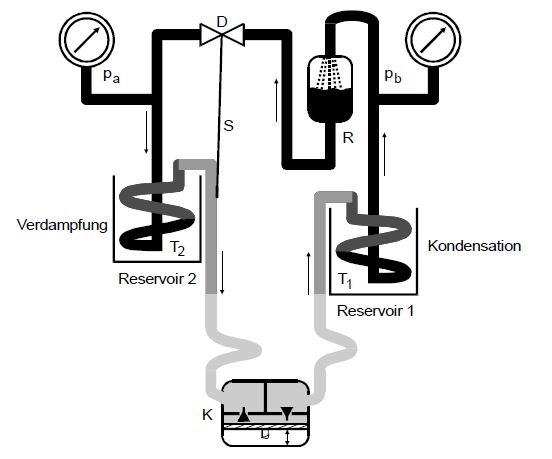
\includegraphics[height=8cm]{Pumpe.JPG}
  \caption{Aufbau einer Wämepumpe ($p_{b}>p_{a}$, $T_{1}>T_{2}$)}
  \cite{skript}.
  \label{fig:pumpe}
\end{figure}
Bei der Temperatur $T_{1}$ und dem Druck $p_{b}$ ist das Gas flüssig, nachdem es das Drosselventil D durchströmt
hat, verdampft das Gas im Reservoir 2 aufgrund des gernigen Drucks $p_{a}$. Dabei wird dem
Reservoir 2 die Verdampfungswärme $L$ pro Gramm Substanz entzogen, also gibt Reservoir 2 die Wärme ab und ist
damit das kältere Reservoir. Im Kompressor, der für eine Mediumskreislauf sorgt, wird das Gas nun
adiabatisch komprimiert, wobei es sich stark erwärmt und aufgrund des steigenden Drucks wieder verflüssigt.
Bei der Kondensation des Gases wird die Kondensationswärme L pro Gramm an das Reservoir 1 abgegeben, wodurch sich
dieses erwärmt.\\
Für den reibungsfreien Ablauf werden weitere Apparaturen benötigt, dazu zählt der Reiniger $R$, der
die übrigen Gasblasen aus dem verflüssigten Gas entfernt, sowie die Steuervorrichtung $S$.
Diese sorgt dafür, dass keine Flüssigkeitsreste des Gases in den Kompressor gelangen.
Außerdem muss die Durchlässigkeit des Drosselventils gesteuert werden, dies geschieht über
die Temperaturdifferen am Ein- und Ausgang der Reservoires 2.

\subsection{Kenngrößen der Wärmepumpe}
Bei einer realen Wärmepumpe sind folgende Kenngrößen von besonderem Interesse:
\begin{itemize}
  \item Güteziffer
  \item Massendurchstz $\frac{dm}{dt}$ des Transportmediums
  \item Wirkungsgrad des Kompressors.
\end{itemize}

Aus dem zweiten Hauptsatz der Thermodynamik folgt unter der Annahme, dass sich die Temperaturen
$T_{1}$ und $T_{2}$ der Reservoire praktisch nicht ändern für den realen, irreversiblen Fall die Relation
\begin{equation}
  \frac{Q_{1}}{T_{1}}-\frac{Q_{2}}{T_{2}}>0.
  \label{eqn:QT}
\end{equation}
Wobei $Q_{1}$ die vom Transportmedium an das wärmere Reservoir abgegebene Wärmemenge bezeichnet und
$Q_{2}$ die vom kälteren Wärmereservoir aufgenommene Wärmemenge.

Eine wichtige Größe zur Beschreibung der Wärmepumpe ist die Güteziffer $\nu$, sie ist definiert
als das Vehältnis der transportieren Wärmemenge $Q_{1}$ zur geleisteten Arbeit $A$:
\begin{equation}
  \nu=\frac{Q_{1}}{A}.
  \label{eqn:güte}
\end{equation}
Mit dem ersten Hauptsatz der Thermodynamik lässt sich $Q_{1}$ als $Q_{1}=Q_{2}+A$ schreiben.\\
Unter der Verwendung von Gleichung \ref{eqn:QT} lässt sich die ideale Güteziffer als
\begin{equation}
  \nu_{id}=\frac{T_{1}}{T_{1}-T_{2}}
  \label{eqn:güte2}
\end{equation}
schreiben. Aus dieser Gleichung lässt sich folgender Zusammenhang folgern:
Je kleiner die Temperaturdifferenz zwischen den Reservoiren ist, desto weniger Arbeit muss
die Pumpe leisten.

Aus der Messreihe $T_{1}$ wird der Differenzenquotient $\Delta T_{1}/\Delta t$ bestimmt,
woraus zunächst eine Relation für $\frac{\Delta Q_{1}}{\Delta t}$ bestimmt wird.
\begin{equation}
  \frac{\Delta Q_{1}}{\Delta {t}}=(m_{1}c_{w}+m_{k}c_{k})\frac{\Delta T_{1}}{\Delta t}
\end{equation}
Hiebei bezeichnet $m_{1}c_{w}$ die Wärmekapazität des Wassers in Reservoir 1 und $m_{k}c_{k}$ die
Wärmekapazität der Kupferschlange, in der sich das Gas befindet und des Eimers, der das Wasserreservoir darstellt.\\
Mit der Größe $N$ als über das Zeitintervall $\Delta t$ gemittelte Leistungsaufnahme des Kompressors
kann folgende Formel für die Güteziffer bestimmt werden.
\begin{equation}
  \nu = \frac{\Delta Q_{1}}{\Delta t N}
  \label{güte3}
\end{equation}

Aus der Messreihe $T_{2}$ wird ebenfalls der Differenzenquotient $\Delta T_{2}/\Delta t$
bestimmt, um folgende Relation zu erhalten:
\begin{equation}
  \frac{\Delta Q_{2}}{\Delta {t}}=(m_{2}c_{w}+m_{k}c_{k})\frac{\Delta T_{2}}{\Delta t}.
\end{equation}
Hier beschreibt $\Delta Q_{2}/{\Delta t}$ die pro Zeiteinheit aus dem Wärmereservoir 2
entnommene Wärmemenge.
Da dem Reservoir die Wärmemenge durch Verdampfen entzogen wird, wird pro Zeit- und Masseneinheit
die Verdampfungswärme $L$ verbraucht. Damit folgt die Relation
\begin{equation}
  \frac{\Delta Q_{2}}{\Delta t}= L \frac{\Delta m}{\Delta t}.
\end{equation}
Wenn die Verdampfungswärem $L $ bekannt ist, kann so der Massendurchsatz $\frac{dm}{dt}$ des Transportmediums
bestimmt werden.

Um die mechanisch Kompressionsleistung $N_{mech}$ zu bestimmen, wird zunächst die
Arbeit $A_{m}$ des Kompressors definiert, die verrichtet wird, wenn ein Gasvolumen von $V_{a}$ zu $V_{b}$
komprimiert wird:
\begin{equation}
  A_{m}= -\int_{V_{a}}^{V_{b}} p dV.
\end{equation}
Für eine adiabatische Kompression gilt:
\begin{equation}
  p_{a}V_{a}^{(\kappa)}=p_{b}V_{b}^{(\kappa)}=pV^{(\kappa)},
\end{equation}
und mit der Definition $N_{mech}=\frac{dA_{m}}{dt}$ folgt für die mechanische Kompressionsleistung
\begin{equation}
  N_{mech}= \frac{1}{\kappa-1}\Biggl(p_{b}\sqrt[\kappa]{\frac{p_{a}}{p_{b}}}-p_{a}\Biggr)\frac{\Delta V_{a}}{\Delta }=\frac{1}{\kappa-1}\Biggl(p_{b}\sqrt[\kappa]{\frac{p_{a}}{p_{b}}}-p_{a}\Biggr)\frac{\Delta m}{\rho \Delta t}
 \label{eqn:Nmech}
\end{equation}
wobei $\rho$ die Dichte des Gases beschreibt und $\kappa$ die Molwärmen $C_{P}$ und $C_{V}.

\label{sec:Theorie}

%\cite{sample}
>>>>>>> michelson
